\documentclass[11pt,a4paper]{report}

\usepackage[utf8]{inputenc}
\usepackage[T1]{fontenc}
\usepackage[italian]{babel}
\usepackage{lmodern}
\usepackage[margin=2.6cm]{geometry}
\usepackage{graphicx}
\usepackage{booktabs}
\usepackage{siunitx}
\usepackage{caption}
\usepackage{xcolor}
\usepackage{microtype}
\usepackage[hidelinks]{hyperref}
\usepackage{float}
\usepackage{tabularx}

\captionsetup{font=small,labelfont=bf,width=0.92\textwidth}
\sisetup{output-decimal-marker={,},group-separator={.},group-minimum-digits=4}
\setlength{\parskip}{0.4em}
\setlength{\parindent}{0pt}
\renewcommand{\arraystretch}{1.25}

\definecolor{autoblue}{HTML}{1f5fa8}
\definecolor{biomedgreen}{HTML}{4a9e6f}
\definecolor{judgegray}{HTML}{6f747b}

\begin{document}

\chapter{Baseline denso biomedico: encoder o retrieval?}
\label{ch:baseline-denso-biomedico}

\section{La domanda}

Nel confronto principale il \textbf{RAG denso} è la configurazione più
debole: la recall dei fatti-gold cresce da \num{0,14} (con \num{100} parole di
contesto) a soli \num{0,39} (con \num{2400} parole), sempre molto al di sotto
del retrieval lessicale e lontanissima dal tetto del GraphRAG (\num{1,00}).
Prima di concludere che \guillemotleft{}il retrieval denso non funziona su questa base di
conoscenza\guillemotright{} occorre isolare la causa. Il divario nasce dall'\textbf{encoder}
--- \texttt{all-MiniLM-L6-v2}, addestrato su testo generico, privo di
vocabolario biomedico --- oppure è un limite \textbf{strutturale} del dense
retrieval su un corpus fatto di fatti brevi e nomi propri (geni, farmaci,
varianti)?

Per rispondere ho sostituito l'encoder generico con encoder di
\textbf{dominio biomedico}, mantenendo identica la metrica --- recall dei
fatti-gold nel contesto assemblato, deterministica e offline --- e lo stesso
sweep di budget dello studio di efficienza di contesto.

\section{Sistemi confrontati}

Il disegno sperimentale separa due contributi spesso confusi: il
\emph{pre-training di dominio} (esporre l'encoder a testo biomedico) e il
\emph{fine-tuning per il retrieval} (addestrarlo a rendere vicine coppie
domanda--passaggio rilevanti). Per questo confronto due encoder biomedici, uno
per ciascun contributo:

\begin{table}[H]
\centering
\begin{tabularx}{\textwidth}{@{}llX@{}}
\toprule
\textbf{Sistema} & \textbf{Encoder} & \textbf{Natura} \\
\midrule
RAG denso (all-MiniLM) & \texttt{all-MiniLM-L6-v2} (384) & generico, retrieval-tuned \\
RAG denso (PubMedBERT grezzo) & \texttt{BiomedBERT} (768, mean-pool) & \textbf{solo} pre-training di dominio \\
RAG denso (PubMedBERT-MS) & \texttt{S-PubMedBert-MS-MARCO} (768) & dominio \textbf{+} fine-tuning retrieval \\
\bottomrule
\end{tabularx}
\caption{I tre encoder densi a confronto. Il PubMedBERT grezzo (masked-LM con
mean-pooling) isola l'effetto del solo dominio; \texttt{S-PubMedBert-MS-MARCO}
aggiunge il fine-tuning contrastivo su MS-MARCO.}
\end{table}

Riferimenti già misurati nello sweep: GraphRAG (\num{1,00} piatto), BM25 e
ibrido.

\section{Risultati}

\begin{table}[H]
\centering
\begin{tabular}{@{}lccc@{}}
\toprule
\textbf{Sistema} & \textbf{\num{100} parole} & \textbf{\num{900} parole} & \textbf{\num{2400} parole} \\
\midrule
\textbf{GraphRAG} & \textbf{\num{1,000}} & \textbf{\num{1,000}} & \textbf{\num{1,000}} \\
RAG BM25 & \num{0,541} & \num{0,835} & \num{0,934} \\
RAG ibrido & \num{0,563} & \num{0,825} & \num{0,889} \\
RAG denso (PubMedBERT-MS) & \num{0,369} & \textbf{\num{0,639}} & \num{0,764} \\
RAG denso (all-MiniLM) & \num{0,139} & \num{0,293} & \num{0,390} \\
RAG denso (PubMedBERT grezzo) & \num{0,017} & \num{0,144} & \num{0,244} \\
\bottomrule
\end{tabular}
\caption{Recall dei fatti-gold nel contesto a tre budget rappresentativi.}
\end{table}

\begin{table}[H]
\centering
\begin{tabular}{@{}lccc@{}}
\toprule
\textbf{Sistema} & \textbf{$\geq$\SI{60}{\percent}} & \textbf{$\geq$\SI{70}{\percent}} & \textbf{$\geq$\SI{80}{\percent}} \\
\midrule
GraphRAG & \num{36} & \num{36} & \num{36} \\
RAG BM25 & \num{144} & \num{251} & \num{575} \\
RAG ibrido & \num{112} & \num{226} & \num{690} \\
RAG denso (PubMedBERT-MS) & \num{669} & \num{1543} & mai \\
RAG denso (all-MiniLM) & mai & mai & mai \\
RAG denso (PubMedBERT grezzo) & mai & mai & mai \\
\bottomrule
\end{tabular}
\caption{Parole di contesto necessarie per raggiungere una soglia di recall.
\guillemotleft{}mai\guillemotright{} indica che la soglia non viene raggiunta neppure a \num{2400} parole.}
\end{table}

\begin{figure}[H]
\centering
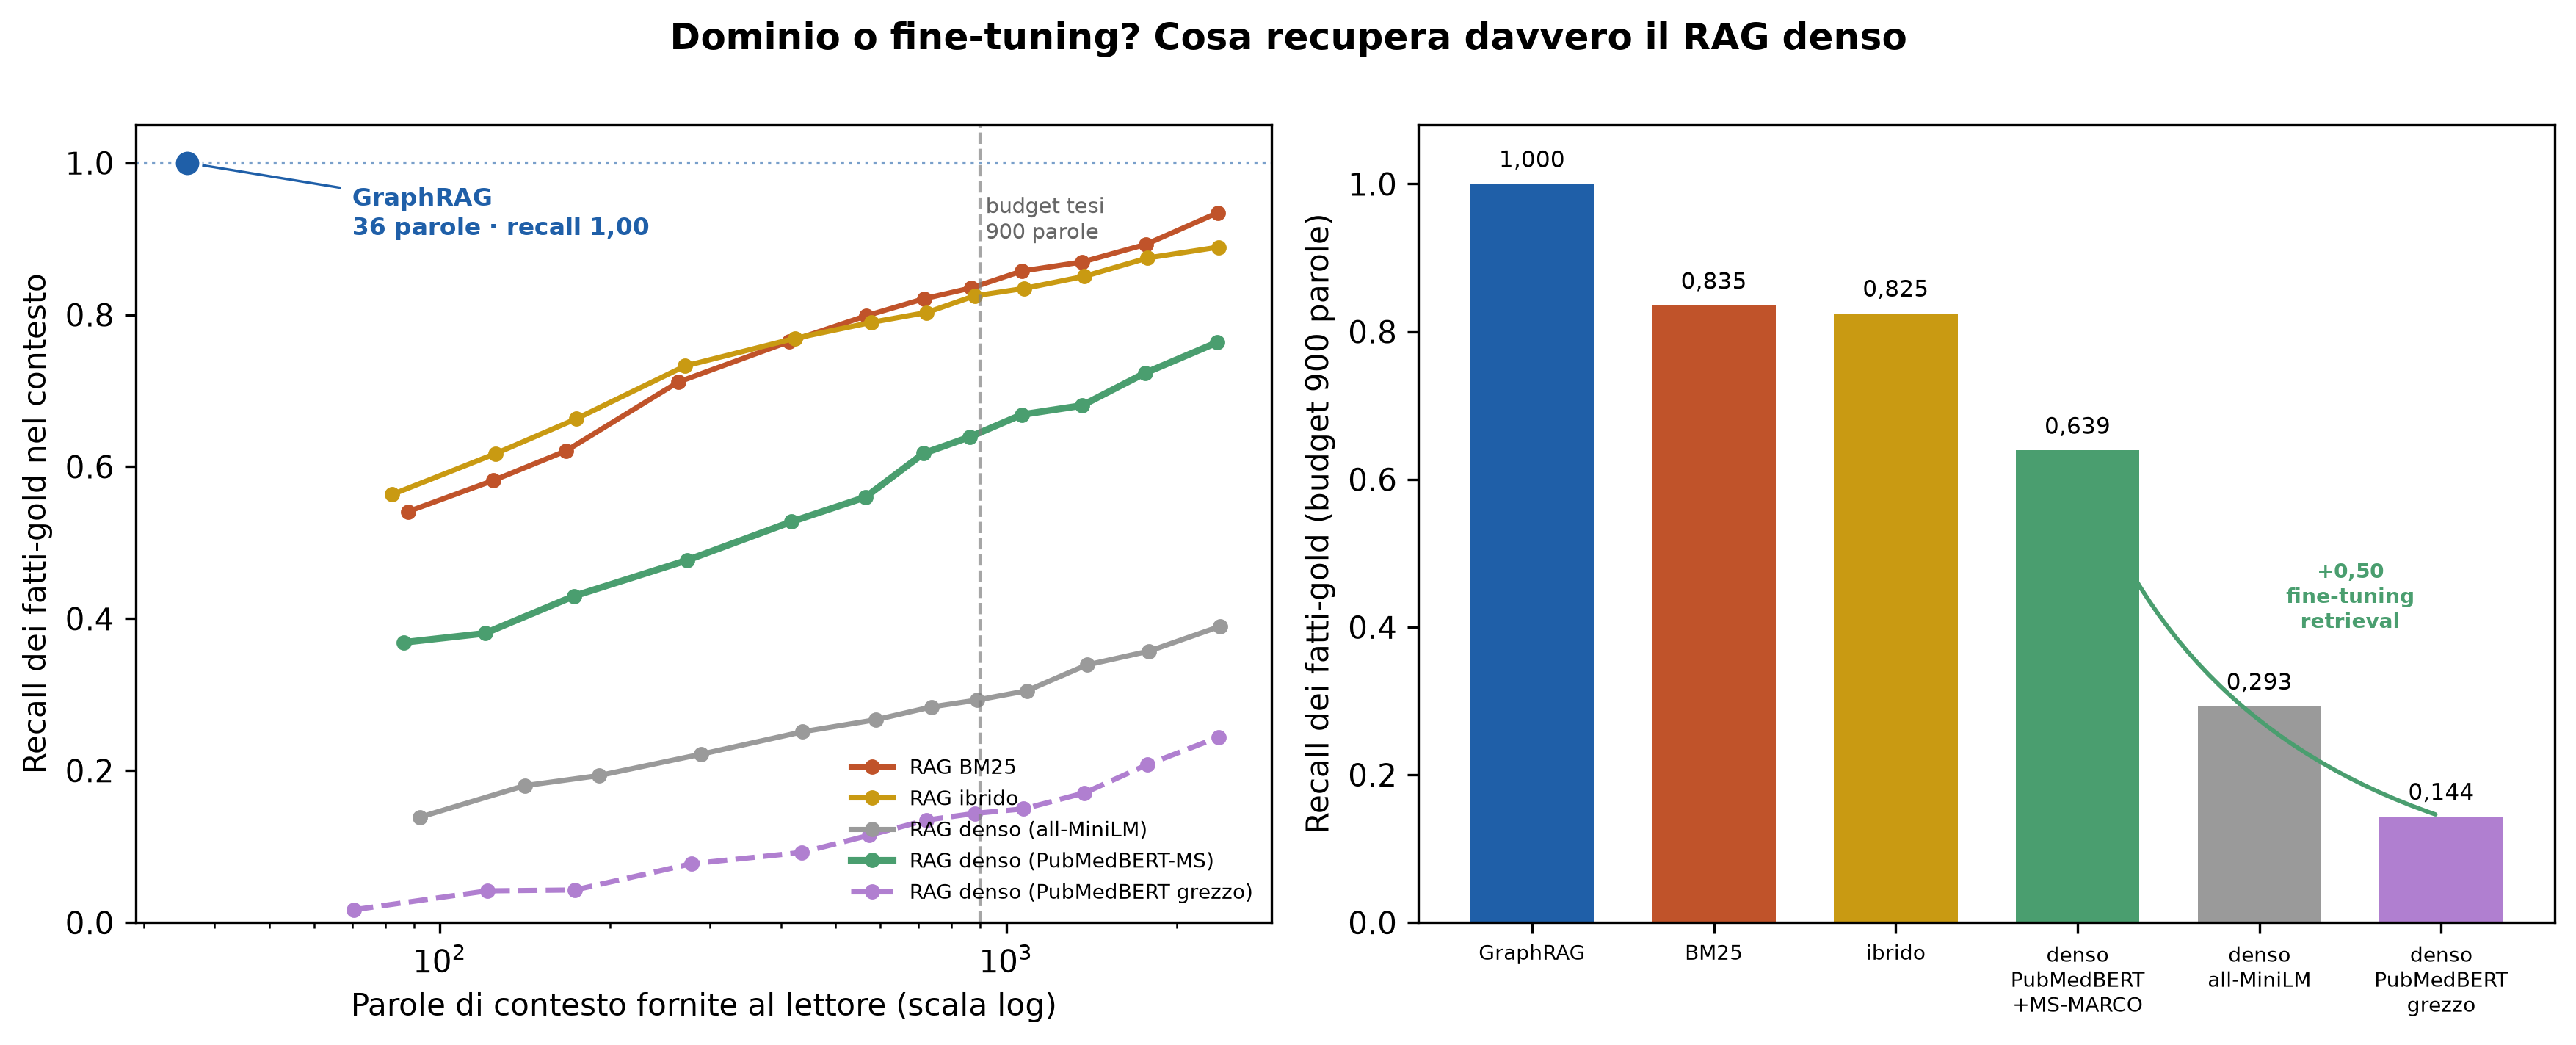
\includegraphics[width=\textwidth]{fig11_biomedical_dense.png}
\caption{\textbf{(a)} Recall dei fatti-gold in funzione delle parole di
contesto (scala logaritmica): l'encoder biomedico retrieval-tuned (verde) si
stacca nettamente dal generico (grigio), mentre il PubMedBERT grezzo
(tratteggiato viola) resta il più basso. \textbf{(b)} Recall a budget \num{900}
parole: il salto da PubMedBERT grezzo (\num{0,144}) a PubMedBERT-MS
(\num{0,639}) misura l'effetto del solo fine-tuning per il retrieval.}
\end{figure}

\section{Tre conclusioni}

\textbf{1. L'encoder biomedico recupera gran parte del divario --- ma non
tutto.} Passando da \texttt{all-MiniLM} a \texttt{S-PubMedBert-MS-MARCO} la
recall a budget \num{900} più che raddoppia: \num{0,293} $\rightarrow$
\num{0,639}. Il denso biomedico supera le soglie del \SI{60}{\percent} (a
\num{669} parole) e del \SI{70}{\percent} (a \num{1543} parole), che l'encoder
generico non raggiunge \emph{mai}. Il divario del RAG denso era dunque in
larga parte un \textbf{artefatto dell'encoder}, non un limite assoluto del
metodo.

\textbf{2. Non è il vocabolario biomedico a contare, ma il fine-tuning per il
retrieval.} Il controllo decisivo è il PubMedBERT \textbf{grezzo}: solo
masked-LM su testo biomedico, mean-pooling, nessun obiettivo contrastivo. La
sua recall a budget \num{900} è \num{0,144}, \textbf{peggiore} persino
dell'encoder generico (\num{0,293}). Il pre-training di dominio da solo produce
embedding inadatti al retrieval; è il fine-tuning su coppie domanda--passaggio
(MS-MARCO) a spostare la recall da \num{0,144} a \num{0,639}. Per il retrieval
conta \textbf{come} l'encoder è stato addestrato, non solo \textbf{su quale}
dominio.

\textbf{3. Anche il miglior encoder denso resta sotto il lessicale e lontano
dal grafo.} A budget \num{900} il denso biomedico (\num{0,639}) non raggiunge
né BM25 (\num{0,835}) né l'ibrido (\num{0,825}); e anche a \num{2400} parole
(\num{0,764}) non tocca il tetto del grafo (\num{1,00}), che il GraphRAG
raggiunge con \num{36} parole. Su una base di conoscenza fatta di nomi propri e
fatti brevi --- dove conta la corrispondenza esatta di un simbolo genico o di
un nome di farmaco --- il retrieval lessicale e quello strutturato del grafo
restano più adatti della similarità densa, per quanto specializzata.

\section{Implicazione per la tesi}

Questo esperimento chiude una possibile obiezione al confronto principale
(\guillemotleft{}il RAG denso perde solo perché usa un encoder generico\guillemotright{}). La risposta è
articolata: un encoder biomedico \emph{retrieval-tuned} recupera buona parte
del divario e va adottato come baseline denso corretto; tuttavia neppure quel
sistema raggiunge la recall del retrieval lessicale, né la compattezza e la
completezza del GraphRAG. Il vantaggio del grafo --- recall \num{1,00} con
\num{36} parole di contesto --- non è replicabile aumentando la dimensionalità
o la specializzazione dell'encoder denso, perché deriva dal \textbf{modo} in
cui i fatti sono collegati, non dalla loro rappresentazione vettoriale.

\end{document}
